\documentclass{standalone}
\begin{document}
	\section{Timing}
	

	One of the highlights of the pipeline is the brief amount of time required to obtain a complete segmentation. To characterize these features, I have performed a benchmark on $5$ CT scans with a different number of slices. For each scan I have performed separately the lung extraction and the labelling step, repeating the procedure several times. The whole test was performed on the server of the Department of Physics and Astronomy. 

	As we have seen, the pipeline operates on the single slice and it is repeated for the whole scan in the axial direction. As a consequence, the time required to segment different scans changes linearly according to the number of slices. To measure the time required to segment a single slice, I have performed a linear fit on the results of the benchmark and I have computed the angular coefficient. 
	 
	\begin{figure}[h!]
		\centering
			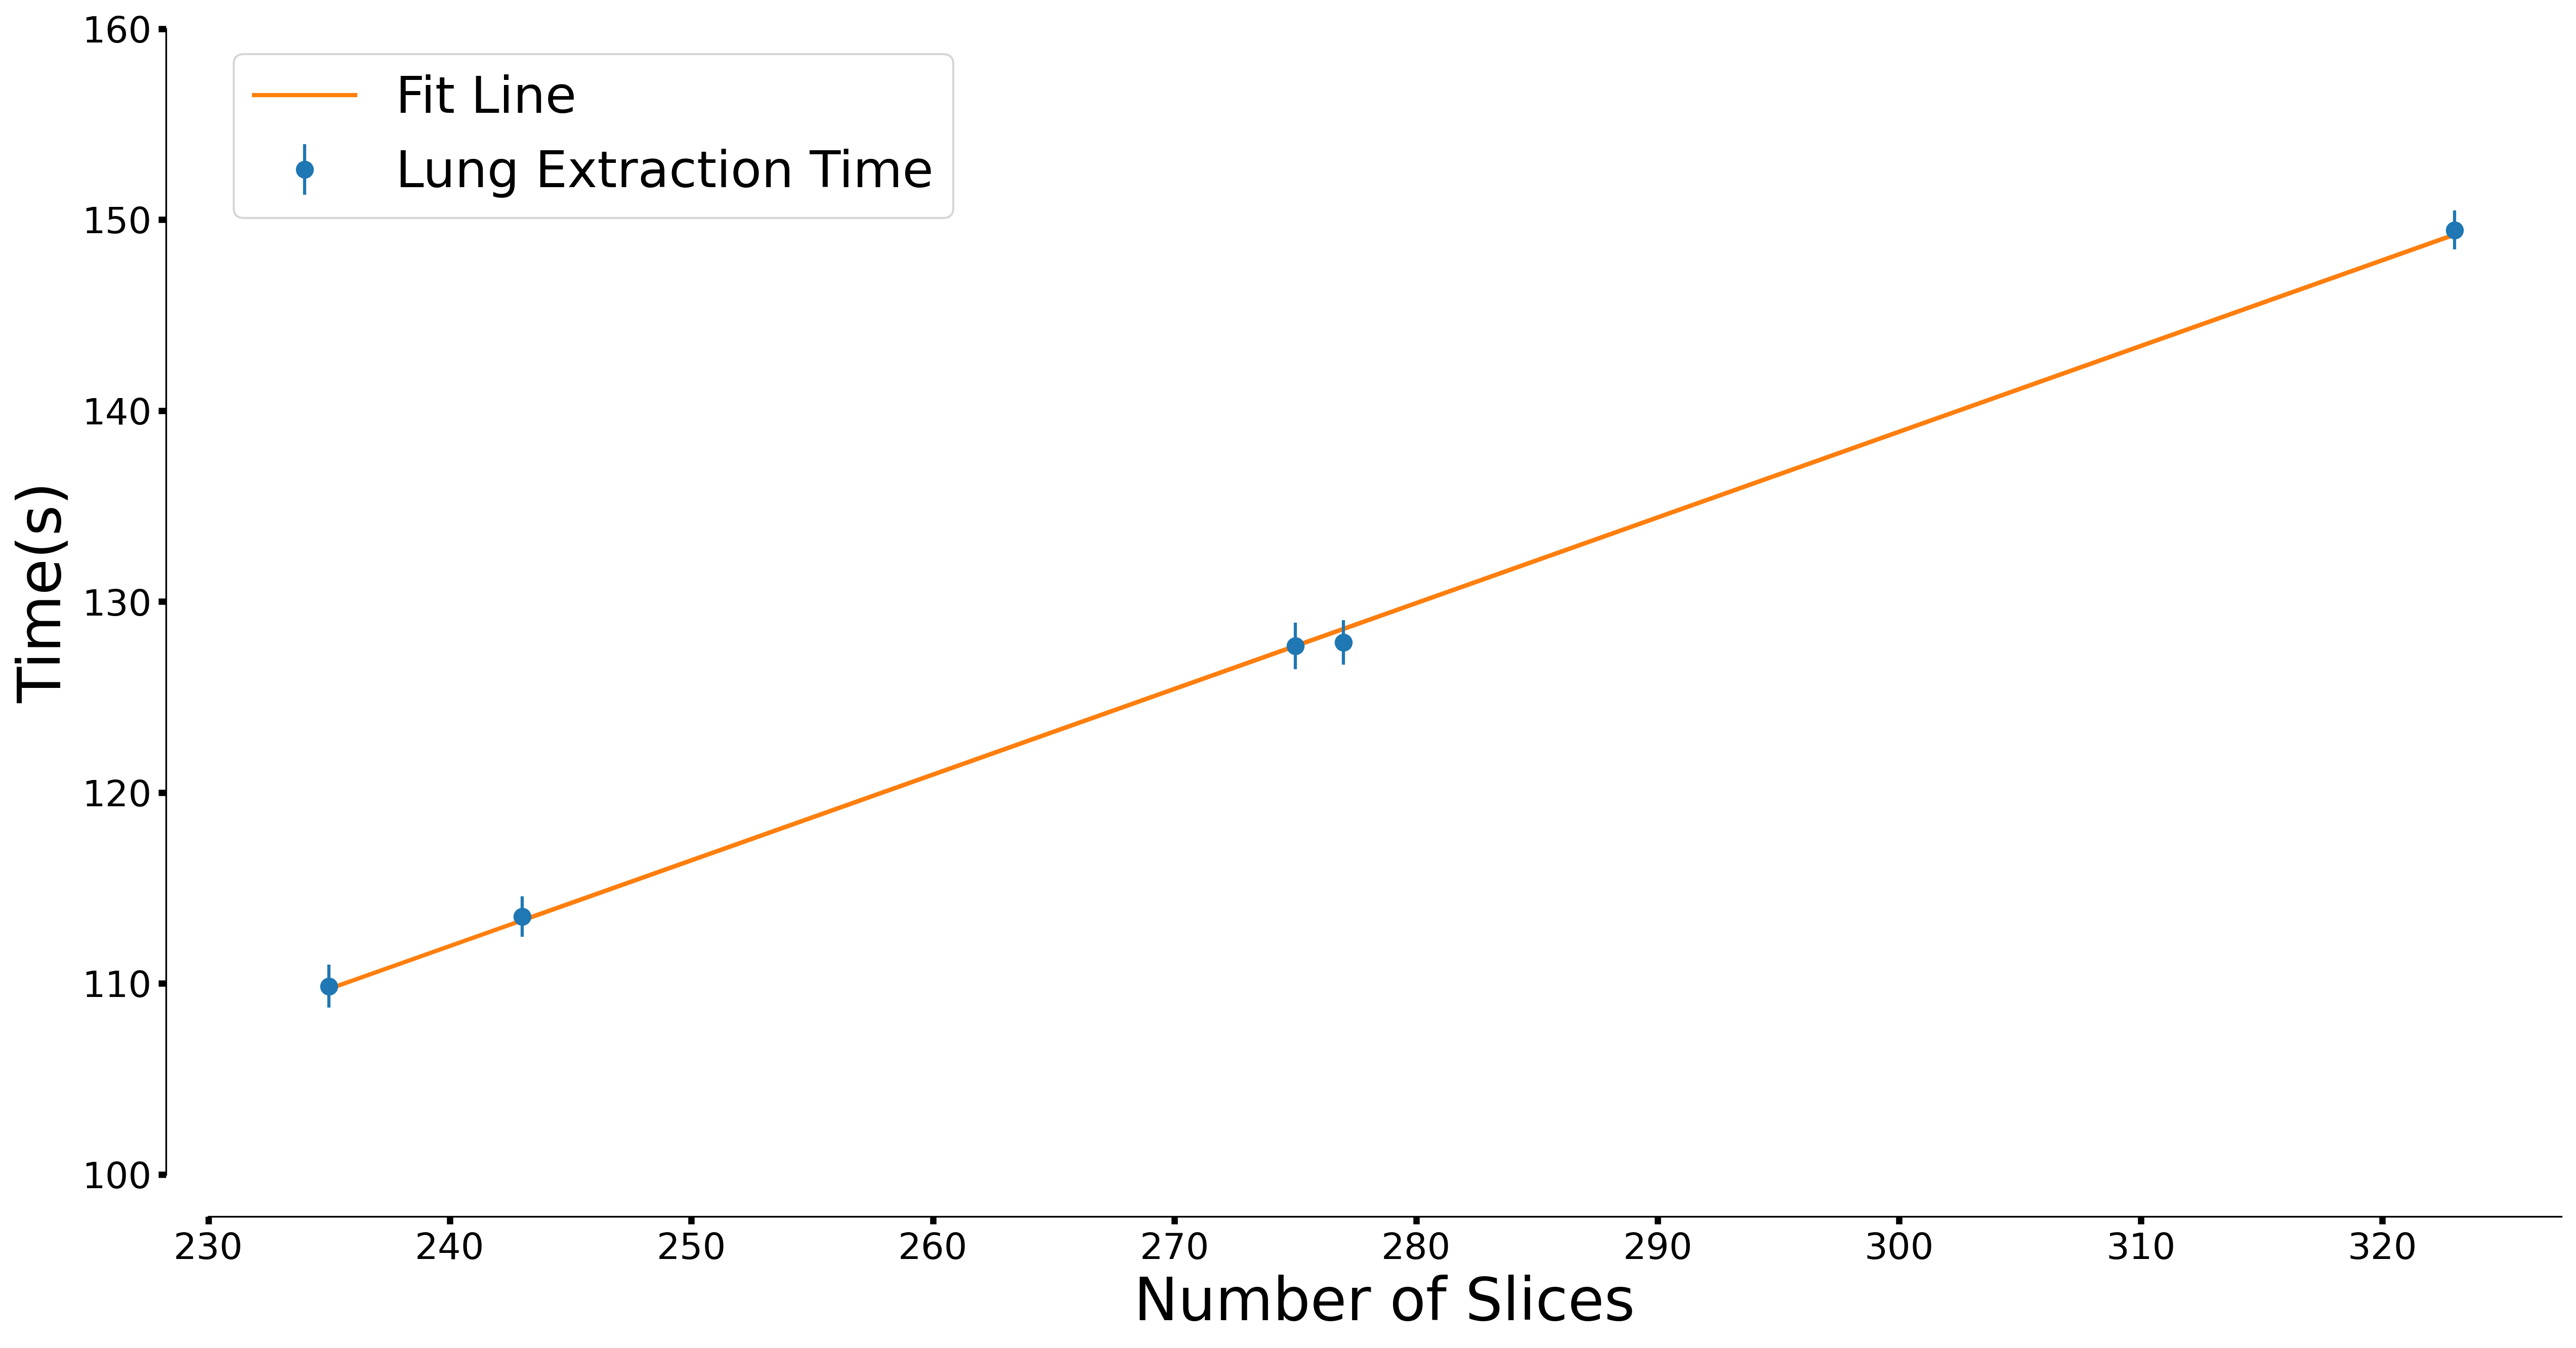
\includegraphics[width=\linewidth]{Lung_timing.png}
			\caption{Lung segmentation time vs the number of slices. We can see that the time required to perform the lung segmentation increase linearly with the number of slices. We can also see that in the worst case the lung extraction requires more or less $2$ minutes.}\label{fig:LungTime}
	\end{figure}

	In \figurename\,\ref{fig:LungTime} I have reported the time for the lung extraction as a function of the number of slices in the scan: as we expected it has a linear trend. In the worst-case, It requires $150\,sec$ to perform the lung extraction. With the linear fitting, I was able to find the time required to process each slice which results: $449.94\pm 0.03\,ms$. We have to notice that these times are acquired without GPU support. Since the application of the U-Net model is performed by \textsc{torch} , with suitable hardware it is possible to parallelize the computing and achieve also lower times.
		
	\begin{figure}[h!]
		\centering
		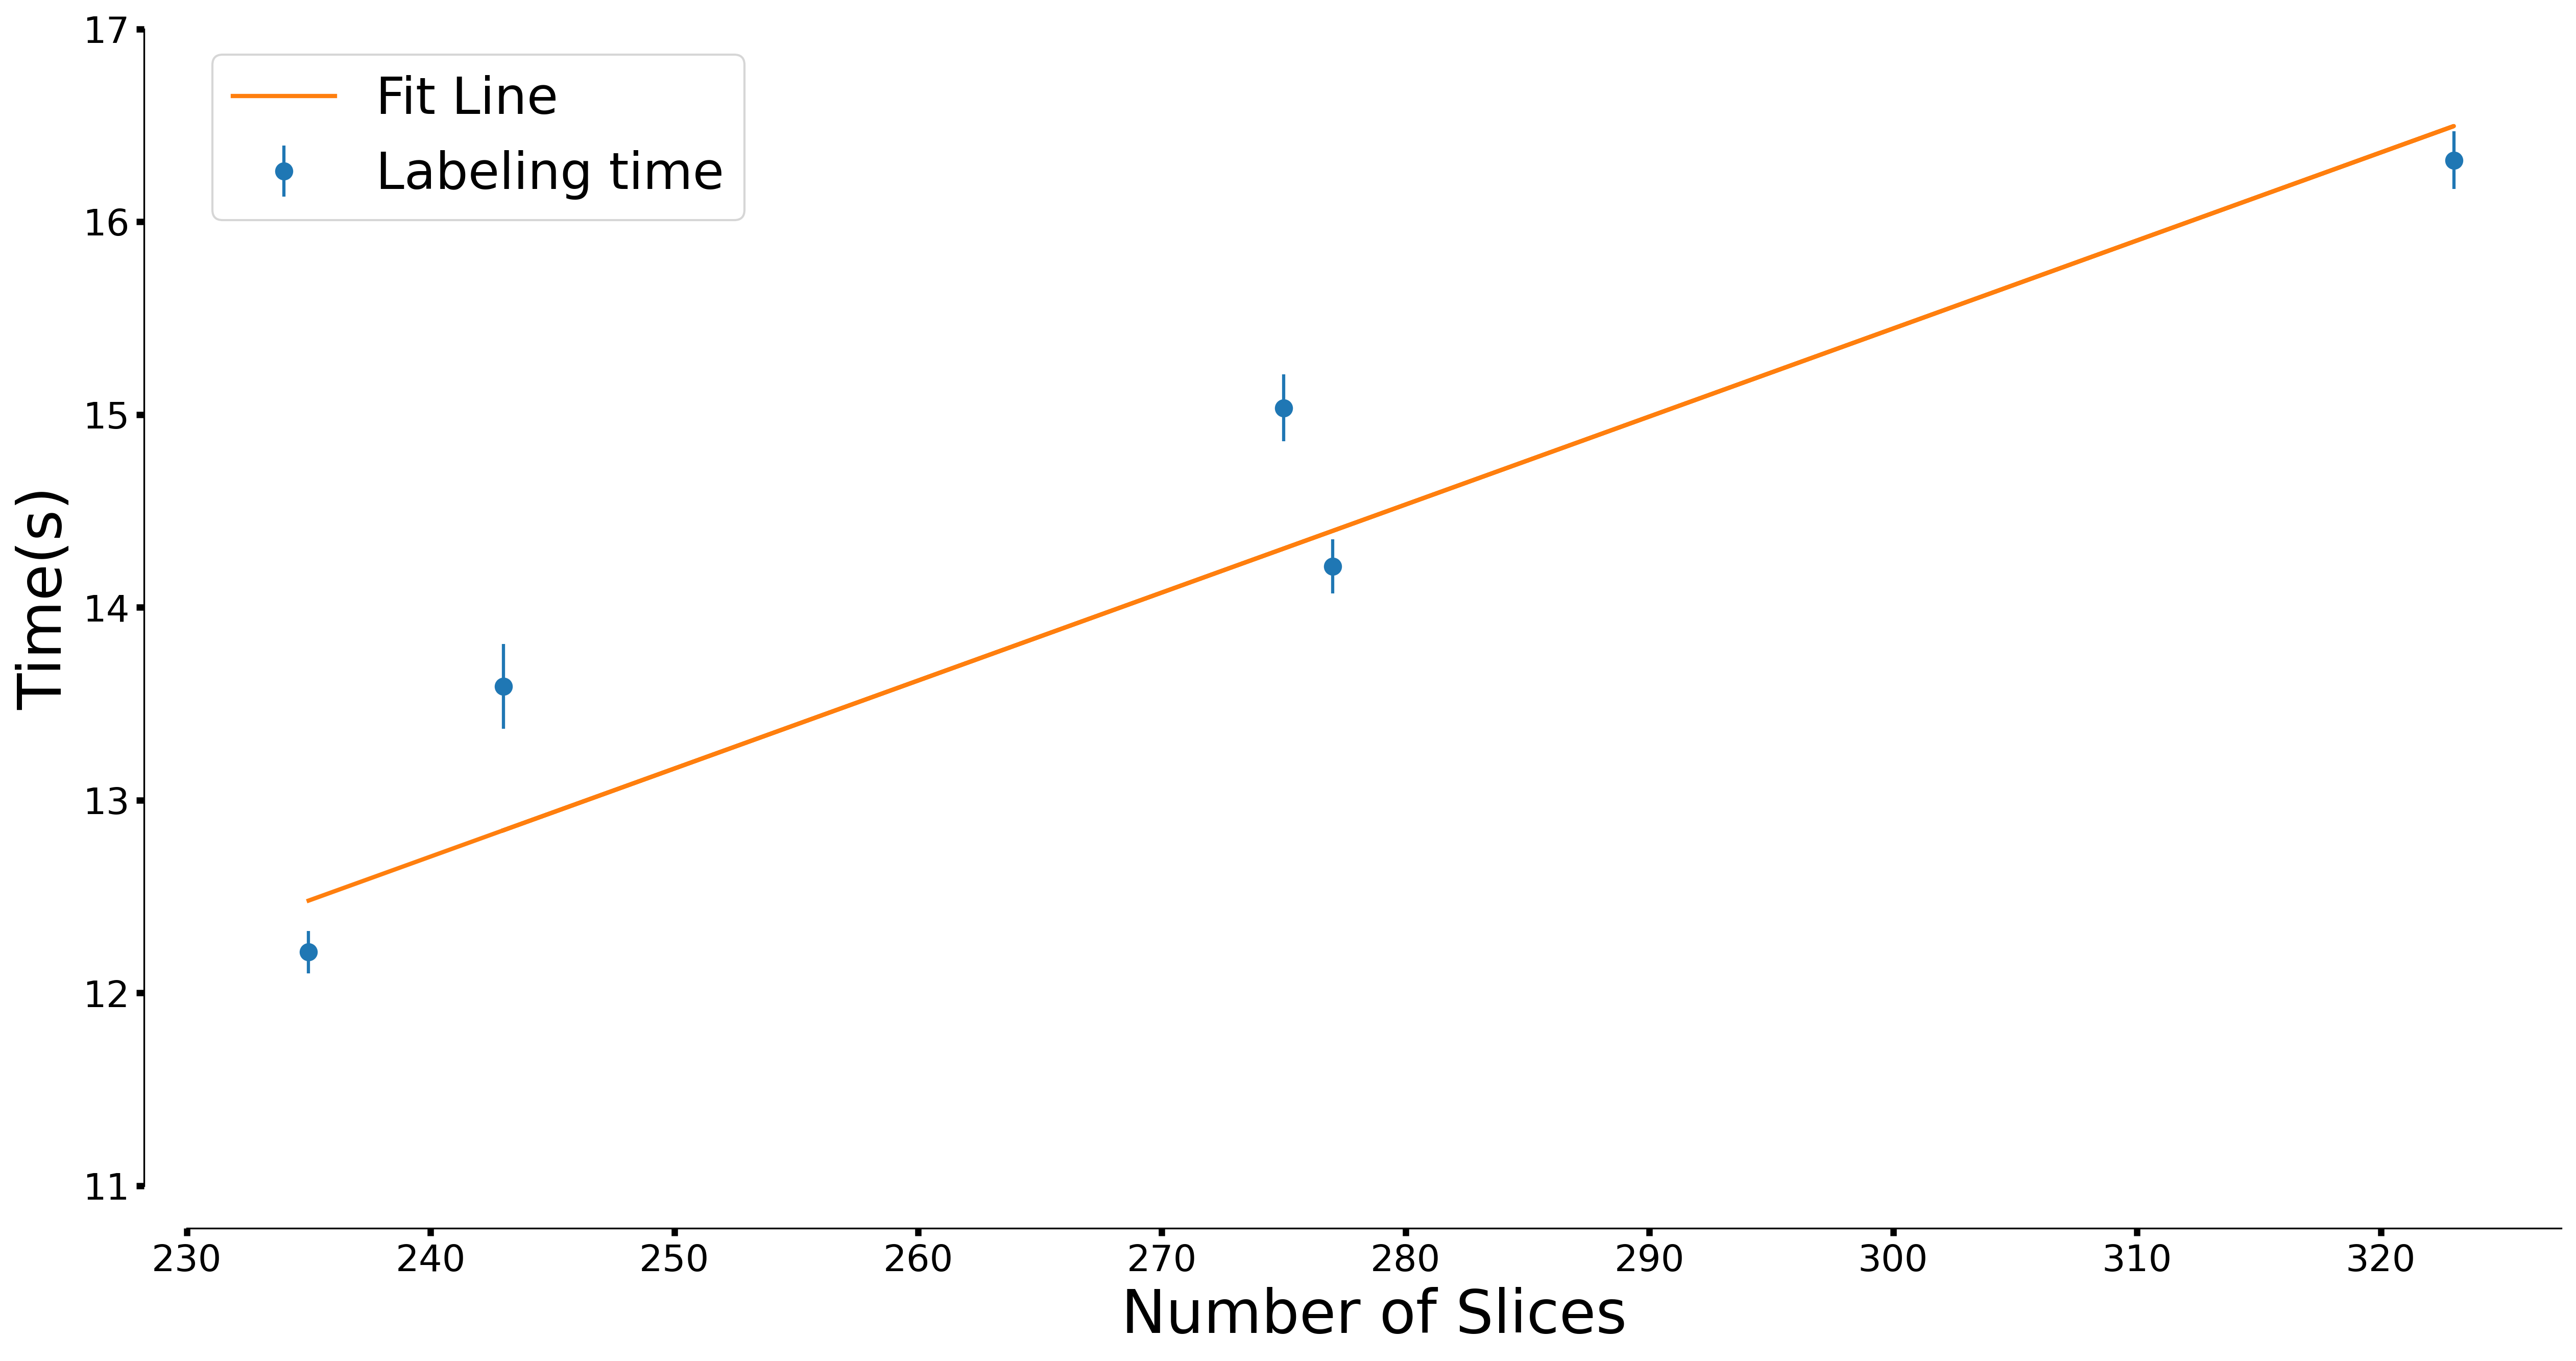
\includegraphics[width=\linewidth]{Labels_timing.png}
		\caption{Labelling time vs number of slice. This time incorporates also the creation of the multi-channel image. As we expected increase linearly with the number of slices and achieve a segmentation in less that $17\,sec$.}\label{fig:LabTime}
	\end{figure}

	In \figurename\,\ref{fig:LabTime} I have reported the results for the labelling. As we can see also, in this case, the trend is linear and in the worst case requires less than $17\,sec$. As before I have measured the time required to label each slice which results: $45.65\pm0.05\,ms$. 
	
	In the end, we have seen that the pipeline achieves segmentation in a low amount of time, which can be further reduced if proper hardware is used.
	
	 
	 
\end{document}